\documentclass[preprint,10pt]{elsarticle}

%% The `ecrc' package must be called to make the CRC functionality available
\usepackage{amssymb}
\usepackage{amsmath}
\usepackage[cmintegrals]{newtxmath}
\usepackage{bm} % optional
\usepackage[latin1]{inputenc}
%\usepackage{amsfonts}
\usepackage{amssymb}
%\usepackage{hyperref}
\usepackage{graphicx}
\usepackage[table]{xcolor}
\usepackage{balance}
\usepackage{tikz}
\usepackage{textcomp}
\usepackage{multirow}
\usepackage{booktabs}
\usepackage{tikz}
\usetikzlibrary{shapes, shadows,arrows}
\usepackage{booktabs} % To thicken table lines
\usepackage{longtable} 
\usepackage{rotating}
\usepackage{threeparttable}
\usepackage{hhline}
\usepackage{tcolorbox}
\usepackage{lscape} 
\usepackage[color=blue!10,textsize=footnotesize,textwidth=35mm]{todonotes}
\usepackage{comment}
\usepackage{url} 
\usepackage{hyperref}


\begin{document}

\begin{frontmatter}

\title{Cross section mergers. Evidence from software industry and implications for research and practice}

\author{Marcin Ocieszak, Krzysztof Wnuk, Emil Numminen}

\address{}

\begin{abstract}
\todo[inline]{WNUK: Why non software need to be software they can develop themselves or buy the competence}
Background: Mergers and acquisitions (M\&A) are two types of corporate takeover strategy, that is widely used for strengthening and maintaining a firm competitive advantage in both domestic and global markets. As digitalization continues to transform many domains, software companies seek for expanding their agenda also outside the software sector. Non-software companies need to face the challenge of becoming software intensive and decide and execute appropriate strategy for this transformation. M\&A seems to be promising as it helps to obtain experience and knowledge rather than grow it. However, the literature lacks investigations about the M\&A announcements across different industries. 

Objectives: The objective of this paper is to analyze the market reactions generated from M\&A announcements between software companies and non-software companies.

Methods: An event study has been used as the main methodology in this thesis. Following the event study, a second-pass regression analysis was conducted in order to explain the event study, by examine the economic impact on the abnormal return derived from M\&A announcements.
\todo[inlne]{WNUK: Say what main results not say that a paper has results}
Results: The result disclosed that target firms tends to experience more positive abnormal returns, while acquiring firms will experience negative abnormal returns. The results of the multiple regression analysis, revealed various significant variables that has high explanatory power to the abnormal return.

Conclusions: We identified the greatest economic impact during an M\&A announcement that involves a cooperative partnerships deals between software target firms and non-software acquiring firms. Furthermore, acquiring firms tends to offer a higher premium to target firms during M\&A transactions. This in turn indicates that acquiring firms will statistically receive less abnormal returns compared to target firms.
\end{abstract}

\begin{keyword}
Economic Impact \sep Event Study \sep Market Efficiency \sep Merges and Acquisitions Announcement \sep Prospect Theory.
\end{keyword}

\end{frontmatter}

%%
%% Start line numbering here if you want
%%
% \linenumbers

%% main text
\section{Introduction}\label{Intro}

\todo[inline]{WNUK: We mainly validate previous research we need to say what is new }
\todo[inline]{WNUK: make the intro shorter, what when and how, what makes this paper novel. The 100 cases analysis is the noverly of the cases. two reasons: increase IT infrastructure for conducting new business and increasing the products they offer, but if these first are mainly speculative capital gain and dividence bying IT infrastructure vs. buying developer }

The software industry has proved to be a vital key and driven factor for changing and evolving our contemporary society. The increased globalization and human interconnection \cite{Pezzi} has accelerated the market growth in software industries. To gain market share and improve competitive advantage in a high-paced software market, lots of companies have resorted to different types of mergers and acquisitions  ("M\&A") \cite{McCarthy}. M\&A can also help to fulfill the following objectives: obtaining existing technology it can be more convenient for a company to utilize existing software and expertise rather than developing something new from scratch \cite{Leger}, instead of launching a new line of business it can occasionally be slightly easier for a company to buy their way into a market \cite{Silva}, improve revenues and profitability through market expansion and product line extension \cite{RAHMAN201524}, eliminate the intensity of rivalry among existing competitors  \cite{Cefis}. As software organizations are not intrinsically restricted to any specific business domain, thus making them a suitable and easy target for M\&As \cite{Pezzi}. Furthermore, software products are becoming more integrated as technology advances, which leads to new emerging and developing markets \cite{chalencon2018cross}. Consequently, the most popular targets in M\&A market, are mostly young software firms.


The software market can provide more opportunities for firms in unrelated business industries to acquire or gain access to a desired software firm, i.e. enabling the options for creating cross-industry alliances ~\cite{Pezzi}. Thus, M\&A is a fitting strategy to adopt with the interest of advancing into a software market, where it can rapidly increase a firm's market power, without having to waste too much time before a business outcome takes effect and produces value ~\cite{schief2012business}. M\&A decisions are strategic decisions to obtain technology, access to expertise or market \cite{AURUM2003945}.

%M\&A usually consist of several steps that could facilitate the process of achieving growth aspiration and a synergy effect of business operation and management  (Zhu, Xia, & Makino, 2015). Yet, depending on the market efficiency, some acquiring firms might follow their own intuitive decisions when selecting a target firm. Whereas the asymmetric economic behaviors can be explained with the help of prospect theory  a decision-making theory that interrelate with behavioral economics.

M\&A transaction for software companies (that product intangible products that are easy to replicate) brings risks that can lead to value destruction across an organization ~\cite{Pezzi}, e.g. uncertain market behaviors, insecure revenues, ambiguous technology dominance, and so on. Hence, there are lots of factors and question that needs to be considered and discussed before adopting M\&A strategies ~\cite{Andriuskevicius}. Despite a wide range of literature reviews of cross-border and domestic M\&A activities, there are barely any literature investigating the economic impacts of M\&A announcements (positive/negative news) across software and non-software industries. With regard to the economic impacts, the finding has also not reached any definite consensus ~\cite{Thathaiah}. Some previous M\&A studies have reported positive effects (wealth gains), whereas some has reported negative effects (losses). For instance, mergers have shown to generate more values for target firms, while an acquiring firm have higher profit chance through an acquisition ~\cite{kashiramka2014shareholders}. 
 

%It is therefore essential for a firm to understand the value of a firm prior to M\&A announcements, as there are various attributes that needs to be considered when selecting a target firm. Such as, what are the characteristics of the technology that is being acquired, e.g. capability, usability, age/longevity, etc. Moreover, based on historical data, how much revenues and profits, and cash flow does a business generate internally from its operations. These elements are important in determining the worth of a business, where the environmental turbulence is high and uncertain ~\cite{Pezzi}.





In addition, there is still a fairly large gap between theoretical findings and successful practical adoptions of M\&As. Especially, regarding economic assessments between firms located in different countries, i.e. whether if geographic distance will create a higher or lower economic impact during M\&A announcements ~\cite{McCarthy}. Since an integration between firms has no clear-cut whether if it creates value or not, it is necessary to increase the synergy that may lead to better performance and value creation in the long run~\cite{Leger}. Another determinant that has scarcely been discussed when valuing a firm, is how essential is a firm's product knowledge within a certain industry, and will ones' own expertise facilitate the process of anticipating the potential profits and benefits of M\&A. Likewise, in the context of M\&A announcements, will the economic impacts be greater or lesser if the product knowledge asymmetry is fair, i.e. depending on if the firms are operating within or outside of the same industry (e.g. software or non-software industry), the economic impacts of the M\&A announcement might differ \cite{McCarthy}. These questions remain relevant for decision makers who either expand outside software industry or would like to obtain products and competences by M\&A with a software company. 

\section{Background, Related Work and Hypotheses}\label{Sec2}



M\&A refers to company takeovers, where a merger is about combining two firms with complementary assets and size, into a new constructed entity. Meanwhile, an acquisition refers to one firm purchasing another firm (i.e. a target firm), which then will be owned by the acquiring firm \cite{vonGersdorff}. The similarities between each process stage for both mergers and acquisitions, indicates that M\&A can be performed with almost the same integration procedures. There are four phases: (i) Consideration - the acquiring and target firm has the time to reflect on why they need to perform a takeover, and envision the future outcome together, (ii) Negotiation - the legal proceeding, where the involved firms will discuss the transaction terms and determines if the takeover will be a merger or an acquisition, (iii) the transaction deal - mostly consist of lots of paperwork (e.g. obtaining approval from government agencies, examine the agreements/contracts, summarize financial statements, etc.), (iv) finalizing the takeover, which in some cases can take several years to complete. This work focuses more on the economic impact generated from M\&A announcements rather than the M\&A transaction itself, the author highly recommend that readers should instead refer to Calipha et al. \cite{calipha2010mergers}, Popp \cite{popp2013mergers} and Schief et al. \cite{schief2013mergers}.

\subsection{Wealth effect around the event day}

From financial perspective the effects of M\&As have been measured using accounting data \cite{Healy,Ghosh} or market data \cite{agrawal1992post}. In the first approach some of the studies prove that M\&As translate into improved operational efficiency, \cite{Healy} other suggest it to be just the opposite \cite{Kruse}, and some do not point to any relationship between the M\&A transaction and their financial performance \cite{Ghosh}. In the second approach, that the articles corresponds literature do not give consistent results, e.g. Yilmaz \& Tanyeri \cite{Yilmaz} has reported positive abnormal returns for both acquiring and target firms whereas Campa \& Hernando \cite{Campa} has reported positive abnormal returns only for shareholders of target firms, and negative abnormal returns for acquiring firms. Nevertheless, these findings of mergers being beneficial only for shareholders of target company seems to be dominant in the literature. 

Also, an interesting point to note, is that acquiring firms tends to have higher risk of receiving negative abnormal returns compared to target firms. As a result of the conflicting claims, many academic research has provide different facts regarding if the effect of M\&A announcements will create or destroy value for a firm's shareholders which has been debated and analyzed within different context area with various cases in the past \cite{Mateev}. In the data sample of Moeller \cite{MOELLER2005533} it was proven that companies paid over USD 3.000 bn for takeovers while the shareholders lost because of these decisions USD 218 bn in market capitalization overall. That is way the M\&As among some researchers are considered as destroying value transactions \cite{bieshaar2001deals,sundersanam2006} what lead to a conclusion that companies behave irrational taking over other company. We investigate these returns for software and non-software M\&As in the following hypothesis.
\\
\\
\textit{H1: Shareholders of target and acquiring companies experience positive abnormal returns around announcement date}
\\

M\&A researchers have been examining different variables that could possibly impact observed abnormal returns. We decided to focus our research on the two main aspects that were not examined when taking into account only targets from software industry.

\subsection{Geographical effect}

Longterm success rate of M\&A in the software market remains low, where in most cases the synergy between companies and the financial outcomes indicates to be less than spectacular \cite{McCarthy}. The software industry consists of a large and varied market, where the competition between firms extends across the globe. Also, the line-of-business operations in the software market are not limited to any human resource or customer relationship, therefore it is quite usual for firms to perform cross-border M\&As especially in software industry.  Having a cross-border alliance means that the resources are shared in a joint headquarter, and is commonly stationed in a different country \cite{ZHU2015556}. This may leads to distributed development challenges, extra costs with on-boarding and other unanticipated issues associated with global software engineering \cite{4221620,vsmite2010empirical}. 

It might not always be the case that an acquiring firm will find a suitable target, that operates within their local geographic boundaries. Consequently, a buyer is then forced to comply, and need to step out of their comfort zone \cite{Huysman}. Country effect can namely be divided into two categories, i.e. domestic M\&A announcement and cross-border M\&A announcement. Which refers to whether if the target firm is located in the same or another country.

Globalization lowers entry barriers for new countries, thus the growth in cross-border M\&A transactions has become more evidently \cite{Mateev} . Since the world is becoming more integrated relative to technology and corporate/economic activities, the purpose behind cross-border M\&As are in most cases about coping with the fiercely international competition that is growing every passing year. Consequently, cross-border partnerships deals accounts for approximately one-third of worldwide M\&A activities, and this figure will certainly keep increasing in the future \cite{erel}. In software industry we observed same pattern over last decades where only 7\% of deals were international in 80s wile 30\% in 10s current age \cite{quo vadis}.

Based on past event studies, there has been different reports regarding cross-border M\&As. For example, while Erel \cite{erel} find acquiring abnormal return to be significantly higher with cross-border target firms (preferably located in a nearby country), other researchers observe a contradictory result \cite{BOUBAKRI20121,andrade}. Yet both of these results are not in line with \cite{Mateev}, which reported no significant difference between domestic or cross-border target firms. Due to the potential benefits with cross-border compared to domestic M\&As \cite{MateevAndovan}, we state the following hypothesis. 
\\
\\
\textit{H2: Shareholders of targets and acquirers experience greater significant economic impact during cross-border M\&As 
compared to domestic}
\\
\subsection{Industry Relatedness}

%Sometime there might be a necessity for a firm to acquire another firm from other industries than their own, due to lack of resources or capabilities (e.g. a software firm may acquire a non-software firm, or vice versa). This strategy is appealing for many non-software companies that transform their daily operations based on digitalization. Merging with a software company, a non-software company gains knowledge that reinforces the absorptive capacity, i.e. ability to recognize the value of new information, and utilize the newly obtained technology or knowledge. -> this is aim of our study, its not the place here

The industry relatedness refers to if whether an acquiring and a target firm operates in the same industry or in different industries. Industry is a prominent factor to examine as the cause of impact on abnormal return during M\&A \cite{ellwanger2015}. A wide range of past event studies have demonstrated similar consensus results in regard to industry relatedness. For example, \cite{scanlon1989,Bley2003,lim2016} find acquiring firms' abnormal return to be significantly higher when a target firm is operating in the same related industry. The reason behind why an acquiring firm is expected to receive a high abnormal return, is that firms in related industry creates better synergy effect and more opportunities to gain market shares \cite{scanlon1989impacts}. The study by  Pierre-Majorique \& Shinkyu \cite{Lger2005NetworkEA} that involved software to software M\&As brings only partially consistent findings. Since our research focuses only on transactions between non software and software companies they are by default only cross section deals. However, close relationship between industries exist and deal between software and software related industries should yield better results than those between unrelated companies.
\todo[inline]{some connection between presented theory and our problem
WNUK: Maybe mention digitalization and that traditional industries are getting more software-intensive like cars, trucks etc.}

By assuming that it is easier to transfer skills and knowledge between firms within the same industry, will indirectly suggest that firms from different industries will underperform. This conjecture is in line with Amewu \& Alagidede \cite{amewu}, who argue that, acquiring a target firm from an unrelated industry will not earn any significant abnormal return for the acquiring firms' shareholders. Gregor and MacCorriston \cite{Gregory} prove that these acquisitions have a negative impact on the wealth of shareholders, explaining  that managers do not know the industry of the company being acquired. Martynova \& Renneboog (2006) \cite{martynova2006mergers} disagreed and concluded that conglomerate mergers, i.e. mergers between firms from different industries will generate higher abnormal returns for target firms' shareholders. We are here also interested in understanding what domains are challenging for software companies to enter via M\&A and why. 
\tood[inline]{WNUK: Here we can write some stories based on the list of companies}
\\
\\
\textit{H3: Target and acquirer will experience greater significant economic impact from the M\&A announcement if the target firm operates in a close related industry}\\

\section{Research Design And Methodology}\label{Methodology}

\subsection{Data}
We extracted raw data of M\&A deals  from the Thomson Reuters database. We decided to limit the data scope to certain remarks in terms of the wide extensive setting of the study to avoid incomplete dataset, i.e. to ensure data availability for each M\&A deal \cite{mackinlay1997}. 

Transactions covered M\&A deals between companies where target has been operating in software industry completed between 1981 and 2018 and acquired did not. We found 1551 deals where target companies were fulfilling the requirements and 10354 where acquiring companies met them. Next, one should have been limit the sample to leave only transaction resulting in change of control following the M\&A. The threshold describing change of control as buying exact \% of shares is different for each individual case and literature did not arrive to any plain conclusions in this matter (from 11\% (Almedia) to even 50\% in case of small private companies). Since no sensible guidelines can be found in the literature during collection process we limited the sample for deal above 5\% and later when performing econometric models we made a robustness checks and prepare models for different level of thresholds.

Since the research focuses on abnormal returns from the stock price we filtered the transactions where acquirer or target were publicly traded companies and so the stock prices were available. Table  \ref{table1}  present the breakdown and data selection statistics.

Should be recalled that there is a huge disproportion between data available for target companies and acquiring in favour of the second group. After considering, however, it seems to be reasonable. Acquirers typically are "the big ones" while targets are simply smaller entities. Since the stock exchange is dominated by the big companies no surprisingly in our database acquirers play the dominant role. To sum up our research consist of two data sets. First, are targets listed on stock exchange (1553 observations), second, are acquirers listed on stock exchange (10359 observations). Depending on the level of threshold when the change of control takes place (5\%, 11\% or 30\%) the available data for our research changes. All further results are presented for 5\% threshold but other levels were examined as well and delivered changeless results.

The target companies were from USA (24\%), Japan (14\%) and Canada (8\%). They were acquired by companies from financial (28\%), IT Consulting (10\%) and alternative financial investments sectors (8\%). All in all, financial sector was dominant as an acquirer taking over about 43,3\% of all targets in a data set. Its dominance, however, was observed only when examining the targets companies. With full


\small
\begin{center}

\begin{table}
  \caption{Summary statistics of database assuming 5\% change of control threshold}
  \label{table1}
  \begin{tabular}{p{1.5cm}p{1cm}p{1cm}p{1cm}p{1cm}p{1cm}p{1cm}}
\toprule
&& \textbf{Targets}& & &\textbf{Acquirers} & &
\midrule
& obs & mean & stdev & obs & mean & stdev\\
AR&859&0,055&0,154&7843&0,001&0,041\\
CAR3&859&0,115&0,243&7843&0,007&0,289\\
DealSize&636&328,2&1733,5&5279&91,425&262,9\\
NetIncome&582&-8,95&811.5&1161&34,6&213,6\\
acquired&859&40,0\%&37,5\%&10359&83,7\%&30,0\%\\
\midrule
\multicolumn{4}{l}{\textbf{Dummy variables:}}\\
domestic&859&76,4\%&&10359&72,1\%\\
finance&856&43,3\%&&10359&8,9\%\\
related&858&26,5\%&&10359&49,1\%\\
merger&859&23,2\%&&10359&23,1\%\\
TFA&859&29,2\%&&10359&18,6\%\\
AFA&859&30,5\%&&10359&14,7\%\\
friendly&859&84,5\%&&10359&94,4\%\\
bubble&859&5,59\%&&10359&19,6\%\\
\bottomrule
\end{tabular}
    \begin{tablenotes}
      \small
      \item TFA states for target financial advisor
      AFA states for acquirer financial advisor
      ARzero is abnormal return in the event day
      CAR3 is cumulative abnormal return in event window three days before and three days after announcement
    \end{tablenotes}
\end{table}

\end{center}



\subsection{Method} 

In order to verify hypothesis we have decided to conduct an event study that analyses the impact on a firm's stock values during public corporate M\&A announcements standardized by MacKinlay \cite{mackinlay1997} implemented by plenty of researchers so far (e.g. \cite{HENDRICKS2003501}, \cite{Fornell2006}).

We defined an event date as a public M\&A announcement. The estimation window consisted of 200 open trading days. The event window covered up to 10 day before and 10 days after announcement however other windows were analysed as well in order to ensure robustness of the results. We assumed market to be semi-strong efficient where the reaction time in the market is immediate and rapid but it might not always be the case that the effect of an event will only last for one day.  Furthermore, choosing a short event window mitigate the risk of getting the data affected by any interruptions (noise) from other corporate actions \cite{LegerYang2005}.

\begin{figure}[h]
  \centering
  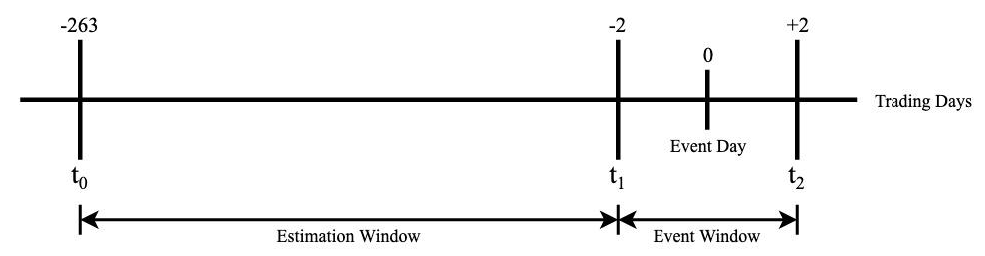
\includegraphics[width=\linewidth] {timline event.png}
  \caption{Time line of the event study}
  \label{Fig1}
\end{figure}


The objective with this event study is to analyze the abnormal returns around the M\&A announcement, i.e. the stock price deviation from the expected return in the pre-defined event window. Where the expected return for each firm was calculated/predicted, by using the ordinary least squares (OLS) to estimate the estimation window.  The normal return is defined as the return that would be expected if the event did not take place. In event studies, one has the privilege of following either a statistical model or an economic model when constructing a normal return model, in order to calculate abnormal returns. In other words, there is no significant benefits using an economic model over a statistical model \cite{mackinlay1997}. Consequently, a statistical model is the more ideal preference in this context.
There are two commonly known statistical models, the constant mean return model that is generally the most simple model of the two, where the normal return is defined as the average return (constant over time) in the estimation window or the market model  which is regarded as a potential improved version of the constant mean return model. Nevertheless, it was found \cite{BROWN1980205} that the results generated from the constant mean return model, and the market model are in fact very similar the market model is more universally used, and is also regarded as one of the most suitable estimation model for event studies. 

Thus, the market model was chosen for estimating the expected return on the stocks, and the Equation as follows \cite{mackinlay1997}:

\begin{equation}
AR = R_{it} - (\alpha_i + \beta_i * R_{mt})
\label{eqn:AR}
\end{equation}
where:\\
AR\_{it} = \text{abnormal return of a firm's stock i on day t} \\
R\_{it} = \text{actual return of a firm's stock i on day t} \\
\alpha\_i = \text{first regression parameter (y-intercept) of firm's stock i}  \\
\beta\_i = \text{second regression parameter (slope/regression coefficient) that  expresses the sensitivity of a firm's stock i to the market index m} \\
E(R\_{mt}) = \text{expected market return on day t}\\


If there is an intention of capturing the overall effect of the event over the event window, i.e. to estimate the total-firm stock movements during a new information and to test the abnormal returns. The cumulative abnormal return (CAR) needs to be calculated. Where CAR is simply the sum of the abnormal returns in the event windows.

\subsection{Measurement variables}

The dependent variable is represented by abnormal return. Consequently, the abnormal return can be used for quantifying an economic impact derived from an event, hence the economic impact reflects the variance of abnormal returns.

Based on the previous research that reported significant difference in abnormal returns for country effect and industry relatedness (see Section \ref{Sec2}), we used dummy variables describing domestic vs cross-border deals and related vs unrelated industry. As related industries we assumed to be (industry according to Thomson Database): computers and electronics, IT consulting, Telecommunications Services, E-commerce / B2B, Internet and Catalog Retailing, Computers \& Peripherals, Other High Technology and Other Telecom.

We used deal and firm related characteristics \cite{Cai2011} as control variables to account for other factors that may change the relationship between the dependent variable and independent variables.  Previous studies has shown promising conclusions finding that acquiring firms earn higher abnormal return if the \textbf{deal size} is large \cite{ALEXANDRIDIS2017}. This result is moderately contradicted by Fuller et al. \cite{fuller2002}, who find that larger target firms will require larger deal, which in turn will create negative impact on the abnormal return of the acquiring firm. This however was supported by Alexandridis et al. \cite{ALEXANDRIDIS20131}, who found that larger target firms generates lower abnormal return if the deal size is also large. Meanwhile, other studies found no significant relation between the abnormal return and the size of acquiring or target firm \cite{CAKICI1996307} .

Whether the transaction of a consolidation nature was so-called \textbf{hostile} takeover or not, is another potential determinant of the effects of consolidation processes. Many studies prove the occurrence of statistically significant positive rates of return due to hostile takeovers for the acquired companies' shareholders (\cite{Lounghran1997}, \cite{Rau1998}), however, in terms of the rates of return for shareholders of companies taking over such a division of transactions is no longer relevant (\cite{FRANKS1996163}, \cite{kini2004}). Among hostile takeovers, takeovers have only the highest returns, with only one hostile bidder \cite{sundersanam2006}.

Acquisitions made by over-valued companies (glamour), which were characterized by high \textbf{financial multiples}, were compared widely, as opposed to transactions of undervalued companies - those with low values of the described ratios. Rau and Vermaelen (1998) \cite{Rau1998} proved that acquisitions made by overvalued companies were characterized by higher rates of return during the transaction announcement period, while much lower during the 3 years after the transaction from other companies. In addition, they confirmed that such glamour transaction for the shareholders of the acquired company are more favorable than for the shareholders of the acquiring company. These results also supported other studies (\cite{sundersanam2003}, \cite{andrade}) giving the same results, however, on other samples. There is, however, inconsistent results in the literature, as a certain group of studies does not confirm the existence of such regularities \cite{mitchell2000}, \cite{dong2006}) and proves that there is no dependence of additional rates of return on whether the acquiring company is overvalued or neither The discrepancy of results is explained by the use of different methods of measuring the phenomenon of overvaluation. The reevaluation of companies is also associated with one of the theories saying that managers of overvalued companies are aware of this, so they protect the interests of shareholders against the fall in share prices that will occur after the bull market, trying to exchange overvalued shares for real acquired assets in the process of mergers and acquisitions (\cite{Gregory}, \cite{SHLEIFER2003295}). This phenomenon is classified by some researchers as issues related to the problem of information asymmetry (\cite{dierkens1991}). In database multiples were included calculating price to different financial position like net income, EBIT, EBITDA, sales or net asset.
Other characteristics that potentially might have had impact abnormal returns were: type of transaction - whether it was merger or acquisition, did target or acquire hire financial advisor, what percentage of shares was acquired and whether transaction took place in dotcom bubble. 

%\textbf{Test Procedure}

%Like many event studies, in order to determine whether if the abnormal returns within an event window are significant different from zero we used parametric and nonparametric tests.

%Given the fact that the market model is a linear regression and normality of the residuals (i.e. the difference between the observed value and the estimated value) is an assumption of a linear model, addresses the choice of using a parametric t-test to test the null hypothesis. A t-test is one of the most common tool within the field of event studies. That provides insight of whether if there is any significant difference (p < 0.05) between two sets of groups, by comparing the means. In other words, t-test determines if a null hypothesis is rejected or not. Which in turn signifies if the difference happened by chance or is reliable. That is, if the same outcome can be found in other assessments with the same data population. For example, in this case a t-test can detect the significance of the abnormal return caused by a M\&A announcement, where the null hypothesis and alternative hypothesis can be defined as following:
%• H0: AR = 0, the abnormal return is not significant different from the expected return (there is no relationship between the groups, i.e. the economic impact is not significant).
%• H1: AR ≠ 0, the abnormal return is significant different from the expected return (there is a relationship between the groups, i.e. the economic impact is significant).
%SOME MATH HERE 

%\textbf{Multiple Regression Analysis}
%3.6 Multiple Regression Analysis
%This thesis study has explored numerous potential independent variables that can explain the variance in the dependent variable. Thus, for the purpose of finding the best well establish relationship between the selected predictors and abnormal return during M\&A announcements, an ordinary least squares linear multiple regression analysis was conducted with the help of the statistical analysis program SPSS. By using a multiple regression analysis it is possible to include two or more independent variables at the same time. Which in turn can help in determine/finding the combination of significant predictors with the highest explanatory power of the variance in the abnormal return. Also, each significant predictor in this case, represents an economic impact on the abnormal return.
%Before commencing a multiple regression analysis, it is essential to create/collect a complete data set (at least as complete as possible). Depending on data availability the number of observation for a regression model will differ. Furthermore, some conditions needs to be met, in order for the data set to be acceptable. Such as, the variables in a regression model complies with the normality assumption (i.e. the residuals are normally distributed, which can be checked with a normal probability plot in SPSS), the independent variables are significant, and tested for correlation/multicollinearity (see more comprehensive description in respective sub-headers above). After the data set and the principle of the multiple regression model has been satisfied, a regression analysis can be carried out. Where the general interpretation of a significant variable in multiple regression analysis goes as following: for one unit increase in the explanatory/independent variable the model predicts that the dependent variable will increase or decrease (depending on the sign on the coefficient) by an amount units, holding all other explanatory/independent variables constant (fixed).


\subsection{Threats to validity}

\textbf{Construct validity}. The main threat to construct validity is associated with our conceptualization of the relationship between stock prices and M\&As. One can question if acquiring a software company follows the same response pattern on the stock market as other companies. Software companies hold mostly intangible resources (software, customer data) that are more difficult to estimate as assets than tangible parts of the companies. We mitigate this threat by discussing the characteristics of software companies involved in the study in the discussion section.

\textbf{Internal validity.} We are aware of additional independent variables or other confounding factors that may have influenced the stock prices for the companies involved in the M\&A process. We carefully selected from the available attributes from the Thomson Reuters database and expand out discussion section with potential uncovered factors. 

\textbf{Reliability.} We ensure traceability by disclosing the sources of data and the extraction rules and the statistical analysis methods applied. 

\textbf{External validity.} We are aware that out dataset may not represent the entire spectrum of software companies and M\&As associated with them. Still, we believe our study provides a comprehensive overiew of the studied problems since we extracted data between 1981 and 2018. It remains an open question how to handle transactions with a lower \% of the shares as a threshold. We leave that for further consideration. 


\section{Results}\label{Results}
\todo[inline]{WNUK: Emil wants to know how many are completed and we need to clear the numbers to do }
%Results H1b and H1b \textit{H1a: Shareholders of target companies experience positive abnormal returns on the acquisition day}
%H1b Shareholders of acquiring companies experience positive abnormal returns on the acquisition day


Table 1 presents the descriptive statistic of the target shares AAR 3 days before and 3 days after M\&A announcement. The largest average abnormal return is observed on the event day (5,57\%) and one day later (3,76\%). These results are statistically significant on the level of 1\% or even 0,1\%. Significant AARs observed one, two or even three days after a deal support our semi strong market efficiency assumption. About 7-10 days after transaction the abnormal returns become close to zero and losing its statistically significance. These findings are in line with literature grounding the conclusions that shareholders of target companies benefit from the transaction (REF, REF, REF).
Worth mentioning is that abnormal returns before transaction are present. By the researchers it is justified by insider trading problem (REF) that apparently is present in software industry like everywhere else.
\todo[inline]{WNUK: Discuss the psychological aspect of paying extra for memories? Emil? }

\small
\begin{flushleft}

\begin{table}
  \begin{tabular}{p{2cm}p{1cm}p{1cm}p{1cm}p{1cm}p{1cm}p{1cm}{1cm}}
  
\hline
\textbf{Target} & \textbf{-3} & \textbf{-2} & \textbf{-1} & \textbf{0} & \textbf{1} & \textbf{2} & \textbf{3}\\



\hline

ARR & 0,31\%& 1,01\% & 1,30\% & 5,57\% & 3,76\% & 0,14\% & 0,08\% \\
Patell Z & 2,00** & 7,57*** & 5,51*** & 50,93*** & 29,19*** & 6,03*** & 5,08***\\
Gen Sign Z & 1,34* & 2,91*** & 2,44* & 8,31*** & 5,55*** & 0,66 & 1,56*\\
Gen Rak T & 0,21& 1,49 & 1,05 & 4,85*** & 4,56*** & ,40 & 1,51\\
positive AAR & 51,40\% & 54,08\5 & 53,26\% & 63,29\% & 58,80\% & 50,24\% & 51,83\% \\
Observations & 858 & 858 & 858 & 858 & 818 & 818 & 818\\
\hline
  
\hline
\textbf{Acquirers} & \textbf{-3} & \textbf{-2} & \textbf{-1} & \textbf{0} & \textbf{1} & \textbf{2} & \textbf{3}\\



\hline

ARR & 0,20\%& 0,13\% & 0,55\% & 1,63\% & 0,26\% & 0,06\% & -0,27\% \\
Patell Z & wtf & wtf & wtf & wtf & wtf & wtf & wtf\\
Gen Sign Z & 0,63 & 1,29* & 3,02*** & 5,01*** & 1,79*** & -2,36*** & -1,54*\\
Gen Rak T & -0,43& -0,12 & 0,71 & 2,59*** & 0,5 & -1,02 & 1,35\\
positive AAR & 48,0\% & 48,7\5 & 50,5\% & 52,5\% & 49,2\% & 44,9\% & 45,8\% \\
Observations & 2374 & 2374 & 2374 & 2374 & 2374 & 2374 & 2374\\
\hline

\hline

\end{tabular}
  \caption{Average abnormal returns of target and acquiring companies.\\ ***, **, * represents 1\%, 5\%, 10\% significance level respectively.}
  \label{table1}
\end{table}

\end{flushleft}

Similar conclusions can be found when analysing Table 2 presenting abnormal returns of acquiring companies. At the announcement date AAR was at its highest (1,63\%) with statistical significance at the level of 1\%. Following days are characterised with lower returns and finally after about 3 days we cannot see impact of merger on shareholder value.


\small
\begin{flushleft}

\begin{table}

  \begin{tabular}{p{2cm}p{1,5cm}p{1,5cm}p{1,5cm}p{1,5cm}p{1,5cm}p{1,5cm}}
  
\hline
\textbf{Targets}\\
\hline
CAAR Type &  CAAR Value & Sample & Patell Z & Gen Rak Z & Gen Rank T & \% positive\\
(-10;10) & 14,74\% & 816 & 266,40*** & 12,14*** & 9,09***\\
(-8;8) & 14,25\% & 818 & 28,88*** & 4,37*** & 8,93*** & 71,3\% \\
(-6;6) & 14,45\% & 819 & 32,55*** & 13,33*** & 9,33*** & 72,16\%\\
(-4;4) & 13,27\% & 820 & 37,52*** & 13,84*** & 9,28*** &  72,7\%\\
(-3;3) & \\
(-2;2) & \\
\\
\hline
\textbf{Acquirers}\\
\hline
(-10;10) & \\
(-8;8) & \\
(-6;6) & \\
(-4;4) & \\
(-3;3) & 2,56\% & 2374 & 8,34*** & 3,88*** & 1,57\\
(-2;2) & \\
\hline

\end{tabular}

  \caption{Cumulative average abnormal returns of target and acquiring companies. ***, **, * represents 1\%, 5\%, 10\% significance level respectively.}
  \label{table1}
\end{table}

\end{flushleft}

On the one hand, acquirers returns are lower, statistically weaker than their targets and the returns sustain shorter. On the other hand, however, acquirers AARs and CAARs are still positive and significant. This findings support hypothesis H1a and H1b stating that abnormal returns around announcement date are positive for target and acquiring company.

\todo[inline]{WNUK: So a discussion point may be that it is better to buy a company than to create your own software development department? How does it look like for non-software buying software?}

Worth mentioning is that findings regarding H1b (acquirer positive returns) are rather in contradiction to the literature since majority of researchers arrived to a conclusion that this returns are negative (REF, REF, REF, REF). 

HERE: Why it is different? Do shareholders believe more in software cross section acquisitions than other industries? Software is sexy than. Acquirers make more rational decisions. Maybe a part of discussion lateron

%Results H2b and H2b 

The hypothesis H2 "Targets and acquirers experienced greater significant economic impact on the event day during cross-border M\&A announcements compared to domestic M\&A announcements" has been accepted in terms of target companies to some extended. We found proofs supporting the hypothesis that domestic transactions influence negatively abnormal returns. For models (2), (3) and (4) the regressor \textit{domestic} was negative -0,089, -0,11 and -0,059 and statistical significant on the level of 10\%, 5\% and 5\% respectively.
When speaking about acquiring companies the results are less straightforward. In models presented in Table X none of the parameters for domestic variable was statistically significant. That is why we cannot accept nor deny the hypothesis, however, lack of observed statistical associations between this two variables is in line with our expectations. 
\todo[inline]{HERE: discussion about internationalisation of software, no borders etc. and since we have services and online stuff we go global when we launch the product}


\setlength{\pdfpagewidth}{8.5in} \setlength{\pdfpageheight}{11in}

\begin{tabular}{lccccc} \hline
 & (1) & (2) & (3) & (4) & (5) \\
VARIABLES & AR & AR & AR & AR & CAR\_3\_3 \\ \hline
 &  &  &  &  &  \\
domestic &  & -0.089* & -0.110** & -0.059** & -0.003 \\
 &  & (0.049) & (0.047) & (0.027) & (0.053) \\
finance & -0.052 &  &  & -0.005 &  \\
 & (0.044) &  &  & (0.029) &  \\
related & 0.023 &  &  & 0.004 &  \\
 & (0.047) &  &  & (0.032) &  \\
merger &  & 0.031 & 0.058 & 0.084** & 0.106** \\
 &  & (0.074) & (0.046) & (0.040) & (0.052) \\
software & 0.004 &  &  & 0.011 &  \\
 & (0.038) &  &  & (0.026) &  \\
targetfinadvisior &  & 0.065 &  & -0.000 &  \\
 &  & (0.059) &  & (0.033) &  \\
ACQfinadvisor &  & -0.011 &  & -0.015 &  \\
 &  & (0.055) &  & (0.031) &  \\
friendlyy &  & 0.031 &  & 0.054 &  \\
 &  & (0.091) &  & (0.051) &  \\
NetIncomeMultiple &  &  &  & 0.000* &  \\
 &  &  &  & (0.000) &  \\
lndealvalue &  & 0.021* & 0.021** & 0.013** & -0.001 \\
 &  & (0.011) & (0.009) & (0.006) & (0.010) \\
acquired &  & 0.000 &  & 0.001 &  \\
 &  & (0.002) &  & (0.001) &  \\
bubble & -0.380*** &  & -0.541*** & -0.006 & 0.650*** \\
 & (0.088) &  & (0.120) & (0.091) & (0.136) \\
Constant & 0.114*** & -0.043 & 0.073 & -0.067 & 0.145** \\
 & (0.039) & (0.108) & (0.057) & (0.065) & (0.065) \\
 &  &  &  &  &  \\
Observations & 336 & 285 & 285 & 263 & 285 \\
 R-squared & 0.060 & 0.062 & 0.120 & 0.175 & 0.088 \\ \hline
\multicolumn{6}{c}{ Standard errors in parentheses} \\
\multicolumn{6}{c}{ *** p$<$0.01, ** p$<$0.05, * p$<$0.1} \\
\end{tabular}



The hypothesis H3 stating that there are significant positive associations between share price performance and industry in which target and acquirers operates returned ambivalent results. On the one hand we did not observed relationship between industry characteristics when speaking about target companies. On the other hand, when examining acquiring companies we can observe that when acquirer is a finance related entity the stock returns yield positve abnormal returns. This phenomenon can be seen in table X, models (1), (2) (3) and (5) where aggressors for variable "finance" are positive and statistically significant.

\todo[inline]{To sum up before we move to conclusions: 1) Mergers influence positively shareholders of targets (in line) and acquirers (not necessarily inline with literature). 2) Domestic deals yields poor results so investors prefer international 3) If acquirer is from finance industry it gives higher returns. All other industry relations that we examined are not relevant.}


\setlength{\pdfpagewidth}{8.5in} \setlength{\pdfpageheight}{11in}

\begin{tabular}{lccccc} \hline
 & (1) & (2) & (3) & (4) & (5) \\
VARIABLES & zero\_w & zero\_w & car33\_w & car33\_w & car33\_w \\ \hline
 &  &  &  &  &  \\
domestic & -0.003 & -0.003 & -0.017 & 0.003 & -0.003 \\
 & (0.003) & (0.003) & (0.019) & (0.010) & (0.007) \\
finance & 0.012** & 0.012** & 0.081** & 0.023 & 0.022* \\
 & (0.005) & (0.005) & (0.032) & (0.019) & (0.013) \\
related & 0.004* & 0.004* & 0.028* & -0.012 & -0.011 \\
 & (0.002) & (0.002) & (0.016) & (0.009) & (0.007) \\
merger & 0.002 & 0.003 &  &  & 0.008 \\
 & (0.003) & (0.002) &  &  & (0.008) \\
TFA & -0.000 &  &  &  & -0.011 \\
 & (0.003) &  &  &  & (0.009) \\
AFA & 0.003 &  &  &  & 0.003 \\
 & (0.003) &  &  &  & (0.010) \\
friendly & 0.002 &  &  &  & 0.000 \\
 & (0.005) &  &  &  & (0.020) \\
lndeal & -0.001* & -0.001* &  &  &  \\
 & (0.001) & (0.001) &  &  &  \\
NetIncomeMultiple & 0.000 & 0.000 &  &  &  \\
 & (0.000) & (0.000) &  &  &  \\
acquired & 0.000 &  &  &  & 0.000 \\
 & (0.000) &  &  &  & (0.000) \\
bubble & -0.001 & -0.001 &  &  & -0.001 \\
 & (0.004) & (0.004) &  &  & (0.010) \\
DealSizeMUSD\_w &  &  & -0.000* & -0.000 &  \\
 &  &  & (0.000) & (0.000) &  \\
NetIncomeMultiple\_w &  &  & -0.000 &  &  \\
 &  &  & (0.000) &  &  \\
Constant & -0.001 & 0.000 & -0.003 & 0.014 & 0.001 \\
 & (0.005) & (0.003) & (0.019) & (0.010) & (0.021) \\
 &  &  &  &  &  \\
Observations & 917 & 917 & 917 & 4,018 & 7,843 \\
 R-squared & 0.015 & 0.014 & 0.013 & 0.002 & 0.001 \\ \hline
\multicolumn{6}{c}{ Standard errors in parentheses} \\
\multicolumn{6}{c}{ *** p$<$0.01, ** p$<$0.05, * p$<$0.1} \\
\end{tabular}


\section{Analysis and Discussion}\label{Discussion}

\todo[inline]{this section is "not touched". So has conclusions copied from Master thesis}
%Event discussion (H1)
Based on presented results, in context of hypothesis H1a and H1b we have summarized that \textbf{in the day of the M\&A announcement shareholders of target company benefit significantly} however we did not find sufficient evidence to support hypothesis H1b that shareholders of acquiring company benefit from the M\&A announcement. This may support a conclusion about irrational acquirers' behaviour and questionable motives of the transactions. On the other hand, this seems to be an indication that the market interprets the M\&A announcements differently, where it can be perceived as either a value destroying or value enhancing impact for the underlying acquiring and target firm's shareholders respectively. This result is in line with  literature \cite{Campa} that states that shareholders of acquiring firm tends to receive negative abnormal returns, while shareholders of target firms enjoy positive abnormal returns. There is a low impact on the abnormal returns prior to the event day which in turn implies that the length of the estimation window is long enough to prevent information leakage. After the event day, the abnormal returns %of acquiring company?? 
drops drastically, where it goes back to its previous original state, as a new information is being incorporated into stock prices rapidly. This implication is roughly consistent with the efficient market hypothesis \cite{fama1991}, since there is a clear indication that an announcement effect is starting to wear off immediately after the event day.

%Determinants discussion
%    - Country effect

 As is seen in Table 4, there is no active significant country effect for neither acquiring nor target firms. These results are in line with Mateev \cite{MATEEV2017}, however, it is quite unexpected that the country effect did not show through in any of the regression models since majority of the studies have reported positive results for domestic and cross-border M\&As (REF, REF, REF). For example, firms that are located in the same country should be able to hold a good communication level compared to cross-border M\&As, i.e. regularly transferring more complete and accurate business information (REF), mitigate the risk of cultural differences (REF), more opportunity to understand the local market (REF), etc. This in turn will make it easier for an acquiring firm to assess a target firm prior to an M\&A transaction. On the other hand, the expectation of cross-border M\&As is, that firms ought be able to extend their market power and expand business diversification that is not available domestically (REF). Nevertheless, a common reason why there is no significant country effect, is that investors argues that the capital market is global (REF). Which means that every country is trading more or less with the same play rules, therefore it makes no difference if the acquiring and target firm is located in the same or different country.

%cross industry effect

The finding is partially in line with Martynova \& Renneboog (2006) who found that conglomerate mergers, i.e. cross-industry mergers will generate higher abnormal returns for target firms. It comes with little surprise that industry relatedness is relevant under theses circumstance, given that an extensive of previous studies has shown different significant results. Where the most common outcome is that acquiring and target firms will more likely gain higher abnormal returns if the involving firms operates in the same industry. The reason for this, as mentioned in the previous chapters, is that operating in the same industry can provide better synergistic effects and create more opportunities for a business to capture market shares. On the other hand, cross-industry carry more risks, and is expected to underperform. Furthermore, firms that decided to invest in diversified businesses, are prone to be subjected to higher agency costs. Which is often caused by managerial self-interest, e.g. managers who refrains from prioritizing value-creation for shareholders, and focus more on diversifying their businesses. Nevertheless, seeing that diversification across different industry prevails, might imply that investors perceive cross-industry as a positive activity.

Consequently, moving along with the fact that the industry relatedness effect is observable, which is simulated in an articulate pattern with the transition of Regression Model 2 to Regression Model 3 in Table 4.9 An interesting perceivable pattern is that the significant variables for acquiring firm are not significant for target firms, and vice versa. With the exception of the non-significant Country variable, other significant variables traits can be interpret as follows: Industry  has a positive significant economic impact on the abnormal return for software target firms. Which indicates that a software target firm will earn a higher abnormal return if acquired by a non-software firm. On the other hand, Deal Size and Revenue  has a positive significant economic impact on the abnormal return for non-software acquiring firm. When a non-software acquiring firm acquires a software target firm, the information regarding the software target firm becomes more active and impactful. As stated by Alexandridis et al. \cite{ALEXANDRIDIS2017}, if the deal size is large then acquiring firms with higher values, e.g. larger revenue will have a higher chance of receiving a positive abnormal return. Moving on, Sales Multiple  has a negative significant economic impact on the abnormal return for non-software acquiring firm. Since, the non-software acquiring firms are the buyers, their investors will most likely have low expectations in future sales. That is, a non-software acquiring firms' revenue growth will not increase for the time being during M\&As. Meanwhile, software target firms will have a positive sign on the Sales Multiple, when acquired by a non-software firm. Whereas in this case, investors of a software target firm might have the mentality of believing that future revenues will increase. As it is shown, that the Revenue variable has become positive for software target firms when comparing Regression Model 2 with Regression Model 3. The next variable is Day Prior Event Premium  which has a positive significant economic impact on the abnormal return for software target firms. As expected, the greater the premium offer the greater abnormal return will a software target firm earn. Since there is an expectation for software target firms to receive a reasonable high premium from non-software acquiring firm, in order for target shareholders to give up their shares. Lastly, the Ebitda Multiple  has a negative significant economic impact on the abnormal return for software target firm. As a normal practice, in order to determining the right premium for a software target firm, a non-software acquiring firm would need to assess the value of a firm. Therefore, different multiple measurements can be used for comparing the financial status between different firms. Moreover, when comparing multiples, it is preferably to compare firms that operates in the same industry, Hence, this might explain the negative signs in cross-industry for software target firms, or that there might be some problems with software target firms' profitability when acquired by a non-software firm.

It seems like that the market reaction in this event study, is consistent with the efficient market hypothesis to a certain degree. Since there is a clear indication in the event window that the stock market is incorporating new public available information in the form of abnormal return, i.e. generated by M\&A announcements. However, some of the prominent variables/factors that was suspected to affect the abnormal return, arrived at some unconventional results in the multiple regression analysis. Such as, the country effect was not in line with either Erel et al. or Boubakri et al. \cite{erel2012,BOUBAKRI20121}. As seen in Table 4, both domestic and cross-border M\&A scenarios showed no significant incremental or decremental explanatory power to the abnormal return, or to any other included variables in respective regression models. This can be depict by comparing Regression Model 1 with Regression Model 2, or Regression Model 3 with Regression Model 4. Where the significant -values for both acquiring and target firms has similar explanatory power, and significance level in respective regression models comparison. On another note, since the Country variable has no effect in any of the regression models, the main focus of this analysis will indirectly be shifted to the Industry variable. The industry relatedness effect exhibited some intriguing results. For instance, due to the industry relatedness effect, an increase in number of significant variables can be identified for both acquiring and target firms in Regression Model 3. Whereas the changeover from Regression Model 2 to Regression Model 3, also presents a noticeable increase in explanatory powers growth for each significant variable. These findings, however, are not supported by literature \cite{scanlon1989,bley2003,LIM2016,amewu}, since there are more significant variables with high explanatory power in Regression Model 3. That is, in cross-industry M\&As both acquiring and target firms can gain higher abnormal returns, compared to the number of significant variables and theirs explanatory power in Regression Model 2. Furthermore, the premium is also higher for target firms in Regression Model 3. This in turn might imply that both acquiring and target firm is under a more influential Winner's curse and Endowment effect respectively.
\todo[inline]{WNUK: start from analysing the reason column and later code the acquirer business description and target business description see the file in the repo}
\begin{figure}
    \centering
    
\includegraphics{ColumnX.jpg}
    \caption{The Deal Purpose for all deal with more than 50 percent of the stock acquired}
    \label{FigThePurpose}
\end{figure}{}

The most common reason was to strengthen operations (93 cases) or strengthen existing operations or expand in primary market (61 cases). Expanding in new o foreign markets was mentioned in only 26 cases, or in new geographical regions in 4 cases. However the possibility to offer new product and services was mentioned in 55 cases. This is interesting \todo[inline]{WNUK: Analyze} 
Next, creating synergies (73) and eliminating duplicate services or operations (73) was frequently mentioned as a reason. 

\section{Conclusion and Future Work}\label{Conclusion}

In summary, the article have analyzed whether if the market reaction derived from M\&A announcements, will generate greater economic impacts on the abnormal return for shareholders of companies that operates in the same industry or in different industries. In order to investigate this phenomenon, an event study has been conducted followed by a multiple regression analysis. Where the time period of announcement dates lasted from 1999 to 2018, which resulted in a total of 144 M\&A announcements. Furthermore, various variables with potential influencing factors on the abnormal return has been brought together to spice up the event study, e.g. country effect, industry relatedness and premium, has more or less been the main focus throughout this work. With the results obtained from the event study, it is safe to infer that target firms tends to experience positive abnormal returns upon M\&A announcements, while acquiring firm will experience negative abnormal returns during the event day.
In the final analysis, few remarks has been pointed out with the intention of gaining new insights from the result tables. Based on the output from the multiple regression analysis, the statistical significant variables are either consistent or inconsistent with past research results. This is interesting to point out, since the findings in this thesis, suggest that the significant variables for respective acquiring and target firms can explains a good portion of the variance in abnormal return. Another intriguing result to point out is that the independent variable for country effect, seems to have no significant explanatory power on the abnormal return under any circumstance. This was an unexpected outcome, since country effect is a common influential variable to include when analyzing the economic impact on abnormal return. Nevertheless, the most prominent effect which the author wanted to behold in this thesis, is the industry relatedness effect. By observing the transition of Regression Model 2 to Regression Model 3 it is possible to identify a clear positive significant explanatory powers growth for each significant variable. That is, both non-software acquiring firm and software target firm will experience a significant increase in economic impact on the abnormal return, in comparison with Regression Model 2. Thus, a conclusion can be drawn, that the greatest overall significant economic impact will occur when a software target firm is acquired by a non-software acquiring firm.
The research question for this thesis is the following: Will M\&A announcements of software acquiring and target firms generate a greater economic impact than a combination of non-software acquiring firms and software target firms? The answer to this research question is as follows: The greatest economic impact will occur with the latter grouping, i.e. when the M\&A announcements consist of non-software acquiring firms and software target firms.
To further emphasize the answer to the research question, the implication of the obtained empirical results can be interpreted as follows: the event study reveals that that there was indeed a significant abnormal return in relation to M\&A announcements on the event day. In other words, this discovery indicates that the abnormal return did not occur by chance, it could in fact be due to the event itself. Furthermore, the results generated from the multiple regression analysis disclosed that the greatest economic impact will occur when the M\&A announcements consist of non-software acquiring firms and software target firms, i.e. in Regression Model 3. As this regression model contained the most number of significant variables with the highest explanatory power to the abnormal return. To be more specific, software target firms will be receiving higher abnormal returns compared to non-software acquiring firms. One of the reason why the Premium variable for target firms has the highest positive significant explanatory power, might be due to the fact that non-software acquiring firms are required/willing to pay a higher premium to software target firms in order to gain a new/existing software technology. As described in previous chapter,10 with the intention of accessing a broader spectrum of technology, and to gain existing relevant technological knowledge through an acquisition, a high premium is inevitable.
When conducting an event study there are many limitations that can be associated with the event study itself, but at the same time there is also a load full of possibilities to customize an event study with a specific objective in mind. Due to the fact that there is actually no mandatory structure to follow, instead there are important steps that one should be aware of when performing an event study. Thus, rather than trying to outline certain limitations that comes to mind, the author will suggest potential improvements and other aspects to consider in future research.

Needless to say, the dependent variable, i.e. in this case abnormal return has countless of different known factors that can influence its value and comportment. However, in most cases, it can be difficult and not recommended to include every factors there is. Therefore, depending on the research topic, some certain variables are more suitable to include and examine than others. For instance, a common known variable that was not embraced in this thesis is the payment method. There are numerous payment methods to choose from during M\&A transactions, such as cash, stock, asset, and mixed payment. Hence, it would be interesting to find out which payment method will generate the highest economic impact on the abnormal return. Since previous studies has opposing views regarding which payment methods is the most beneficial, where a payment method can also represent the wealth of a firm's shareholders. Therefore, by including payment methods in an event study, it might be able to facilitate the process of valuing a company prior to M\&A activities. Although the payment method variable has been included in various past research studies, the context related to non-software and software firm remains scant. Hence, the author propose that in future research that are similar to this thesis topic, should include the payment method variable. Where the purpose could be to determine if an acquiring or a target firm will earn more abnormal return for their shareholders depending on which payment method is being used.

Another suggestion of future work is to investigate whether if the experience of an acquiring firm has a positive effects on acquisition performance. That is, if a firm with prior/more acquisition experience, will perform better acquisitions compared to firms with limited acquisition experience. The term experience in this case may refer to factors that can be of advantage for an acquiring firm to benefit from/with in subsequent acquisitions. Such as, is there any significant relation between previous learned knowledge of acquisition deals, and acquisition performance. Where previous learned knowledge can be represented as, for example, number of previous acquisition deals, deal size similarity, etc. Which in turn might have some statistical explanatory power that can explain/affect acquisition performance, where performance might also as well be estimated/measured as abnormal returns. This recommended future approach, is an interesting area to investigate. Since acquisition experience plays an important role when it comes to strategic investment planning and valuation regarding business takeovers. Additionally, acquisition experience might also be able to facilitate the process of an acquisition, or even serve as a motivation for an acquiring firm to acquire a target firm outside of their own comfort zone. That is, acquiring a target firm that operates in another industry, e.g. software or non-software industry. Hence, it would be interesting to investigate and determine whether if acquiring firms with more experience, can generate more value during an event of acquisitions.

% more complex set of determinants

%% The Appendices part is started with the command \appendix;
%% appendix sections are then done as normal sections
%% \appendix

%% \section{}
%% \label{}

%% References
%%
%% Following citation commands can be used in the body text:
%% Usage of \cite is as follows:
%%   \cite{key}         ==>>  [#]
%%   \cite[chap. 2]{key} ==>> [#, chap. 2]
%%

%% References with BibTeX database:

\bibliographystyle{elsarticle-num}
\bibliography{refs}

%% Authors are advised to use a BibTeX database file for their reference list.
%% The provided style file elsarticle-num.bst formats references in the required Procedia style

%% For references without a BibTeX database:

% \begin{thebibliography}{00}

%% \bibitem must have the following form:
%%   \bibitem{key}...
%%

% \bibitem{}

% \end{thebibliography}

\end{document}

%%
%% End of file `ecrc-template.tex'. 
